\chapter{Properties and Applications of Audio}

% The study of sound effects dates back to bbc-years book
The use of sound effects has a long history, already in 1931 certain sound effects were used for their evocative ability to bringing up strong memories, images, or feelings in the mind \parencite{bbc_yearbook_1931}.

% Theory from earcons and icons, as the base building blocks for sound feedback

\section{Properties} 
I will start by introducing the the basic attributes of sound, which will be helpful for the further discussion. First of all, sound are audible waves of pressure traveling trough a medium, and emitted by a vibrating object. The range of audible frequencies depends on the species, for humans it is usually 20 Hz to 20 kHz. Frequency of the sound defines its pitch, higher and lower pitch correspond to higher and lower frequency, respectively. A tone is a sound with a certain pitch The lowest frequency of a vibrating object is called the fundamental frequency (indicated as f; Fig. \ref{fig:fundamentalfrequencyandharmonics}). Its positive integer multiples are called harmonics (indicated as 2f, 3f, and so on). The fundamental frequency is also called the first harmonic. Pressure waves with higher frequency than that of the first harmonic, but not its positive integer multiples, are called overtones. A musical tone (a steady periodic sound) can have the same fundamental frequency, duration, and loudness, as another tone, but have a different feel. For example, consider the same melody played by a banjo and a guitar. They will feel differently due to an attribute called timbre (or tone color) \parencite{noauthor_fundamental_nodate}. \parencite{blattner_earcons_1989} write: "the timbre of a sound is usually described with adjectives such as bright, warm, harsh, hollow, twangy, or brassy". A sound that comprises of one sine wave, only its fundamental frequency, is timbreless, "the sine wave lacks timbre in the same sense that white lacks color" \parencite{blattner_earcons_1989}.
% different instruments have different timbre (i.e. a banjo and a guitar); timbre == tone color
% TODO: what is sound (waveform), fundamental frequencies, timbre, harmonics, and overtones

\begin{figure}
	\centering
	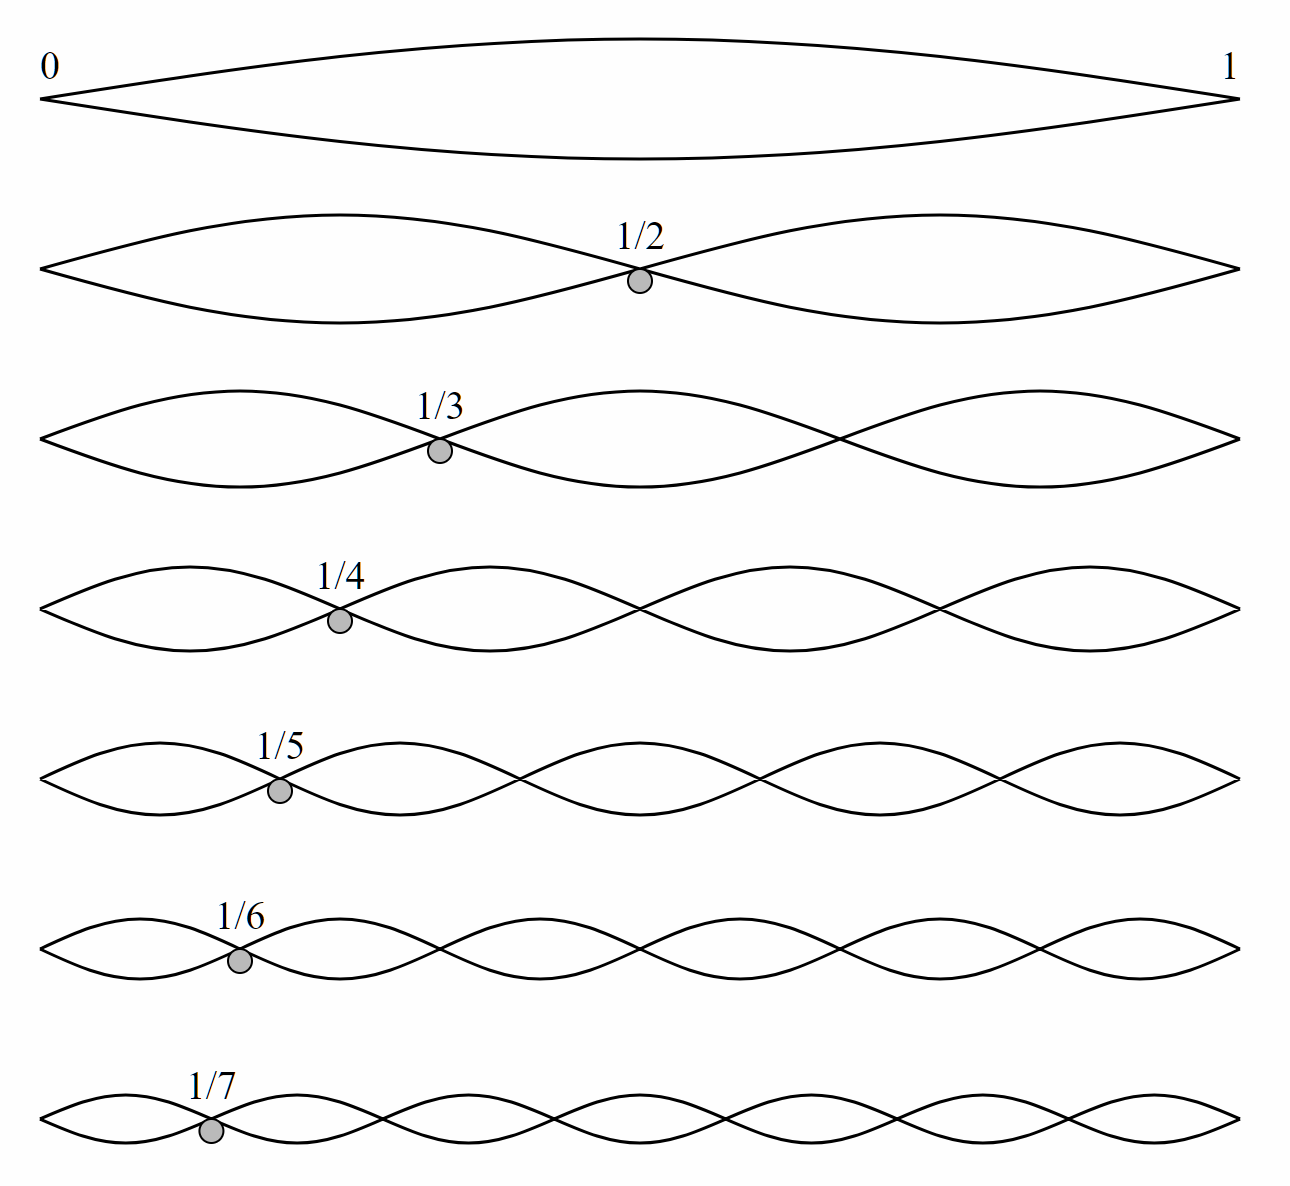
\includegraphics[width=0.7\linewidth]{figures/placeholders/fundamental_frequency_and_harmonics}
	\caption{Fundamental frequency and its harmonics (redrawn from \parencite{noauthor_fundamental_nodate})}
	\label{fig:fundamentalfrequencyandharmonics}
\end{figure}

\parencite[p.~46]{jr_3d_2017} argue that the auditory sensory system is the second-most used sensory channel after the visual channel . As with the visual system, the auditory system provides us with different localization cues that allow us to determine the direction the sound is coming from and distance to it. The main types of \textit{auditory cues }are:
\begin{description}
	\item[binaural cues] - the direction of the sound source is derived through comparing the sound waves received at each individual ear. The limitation of binaural cues is that there are certain positions around the listener, where the cues are ambiguous and it is not possible to uniquely identify the direction;
	\item[Head-Related Transfer Functions (HRTFs)] - spatial filters that are applied to the original sound when it goes through the listener's torso, shoulders, head, and the outter ears. The latter contain different notches and grooves that elevate of suppress sound depending on which direction it came from. HRTFs help solve ambiguous cases caused by binaural cues;
	\item[reverberation] - the collection reflected sound waves from the surfaces in the environment. Besides providing the listener with spacial information about the layout of the environment, reverberation allows them to determine the distance to the sound source;
	\item[sound intensity] (loudness) - the primary cue in determining the sound source's distance. It is also a very simple cue to implement.
\end{description}
The authors also note that auditory cues combined with visual cues can be used to form better spatial perception of the environment. Additionally, the familiarity with the environment can influence the listener's ability to locate the sound source.

Another important aspect for presenting the aural information to the listener is the selection of an \textit{auditory display} \parencite[p.~153]{jr_3d_2017}. It defines in which way the audio is synthesized, how it is presented to the listener % TODO: do you mean the medium?
, and the ways in which the auditory cues are used in the application.
Different approaches to audio synthesis (i.e. using mathematical models, or sound sampling) have direct influence on the resulting auditory cues. For example, in case of taking HRTF measurements during sound sampling, this is usually done in echo-free environments, therefore, the recorded sound is stripped of the reverberation effect. This influences the perception of distance to the sound source

The authors point out several different ways in which audio displays can be used:
\begin{description}
	\item[localization] determining the direction and location of a sound;
	\item[sonification] turning information into sounds;
	\item[ambient effects] adding realism and the sense of immersion in a 3D application;
	\item[sensory substitution] playing a role of another perceptual cues (i.e. emitting a sound instead of haptic feedback); 
	\item[annotation and help] providing additional guidance in the environment (i.e. recording vocally indicating the correct way, or the auditory annotations of a previous user about an artifact in the shared environment).
\end{description}

\section{Sonification for Monitoring}
\parencite{hermann_sonification_2011} argue that sonification has great application in monitoring. While it might seem to be a part of the localization task, cognition is also required for monitoring, not just perception of the sound source - users must understand what the emitted sound conveys.

% Monitoring
One of the problems with auditory displays is that they are a temporary medium, that is - not available for immediate review at any given time. The authors argue that this is the exact reason that makes auditory display a perfect match for the monitoring task, as it is often carried out as a secondary task in parallel with one or more primary tasks, and is based on paying attention to the temporally-related changes to the state of the system.

% Types of monitoring
Monitoring can be classified into two types: \textit{information pull} (\textit{direct monitoring}) and \textit{push}. The former is the case, when monitoring is a primary task and is attended by the user intentionally, the latter treats it as a secondary task, and therefore the information has to be "pushed" into the user's attention space. The push category can be additionally substituted into \textit{peripheral} and \textit{serendipitous-peripheral monitoring}, depending on the role the information plays for the primary task: important or just a convenience (serendipitous) role, respectively.

% Modes of listening
Human hearing can also be classified in several different ways. If we use the push and pull analogy, \textit{hearing is a push} activity, where sounds are forced onto the listener, and \textit{listening is a pull}, where the listener is intentionally attending to the information being conveyed through sound \parencite{hermann_sonification_2011}. Other classifications categorize listening based on the attention to different properties of sound. In this way, \textit{everyday} (or \textit{casual}) \textit{listening} refers to the activity, where attributes of the sound source are being attended: "\textit{big} lorries, \textit{small }children, \textit{plastic }cups being dropped, \textit{glass }bottles breaking", etc. On the other hand, in \textit{musical} (or \textit{reduced}) \textbf{listening}, humans attend to the attributes of the sound (pitch, intensity, timbre, and so on). \textit{Semantic listening} mode involves interpretation of the message encoded in the sound. In this way, the same vocal message with different "muscial" properties can be interpreter equally.

% Some interesting systems (AR-Kola)
% ...

% Pitfalls - annoyence and stuff
There is a number of pitfalls when designing auditory displays, most of them can be classified into either \textit{intrusion and distraction, fatigue and annoyance}, or \textit{audience related sonification problems}.
% intrusion and distraction, fatigue and annoyance
The former mainly explores the trade-off between intrusiveness of the sound and the communicating enough information. \parencite{hermann_sonification_2011} reviews the different ways that were previously employed in an attempt to tackle this problem. For example, sounds that fit to the working environment ecologically, like ticking clock in the office environment, can be less intrusive due to the fact that they correspond to the listener's expectations of the environment. However, non-intrusive sounds lose their perceived importance for the listener. To tackle this problem, the minimal intrusion can be intentionally imposed by variable speed, timbre, or intensity of sound to simultaneously draw listener's attention, and not obstruct the work too much.

%% Audience based: emotional associations, auesthetic and acoustic ecology (allowing users to choose the ecology), and comprehesibility and audibility.
There can be different audience related sonification problems, \parencite{hermann_sonification_2011} reviews three: \textit{emotive associations}, \textit{aesthetic and acoustic ecology}, and \textit{comprehensiveness and audibility}. Different users require different information from the data, and emotive association accounts for that. It describes the problem of presenting information that is too detailed to the parties that do not need it (i.e. sonification of the weather reports for meteorologists and average consumers should be yield different results). Aesthetic and acoustic ecology corresponds to the idea of combining compatible sounds in an auditory display (in terms of frequency and intensity balance, correspond to the same theme, and take the cultural and personal differences of the audience into account. Comprehensiveness and audibility of auditory cues can be highly dependent on the social and cultural norms, and therefore have to be designed with the listener target group in mind.
% TODO: put sound ecologies in the possible future work, if more sounds were to be added they should be competible

\paragraph[]{Earcons and auditory icons}
The last topic I will review in this chapter concerns different ways of sonifying information. \parencite{blattner_earcons_1989} review earcons, the aural analogy of a visual icon (i.e. desktop icons in Windows or Mac OS), and divide them into three groups, in alignment with previous research on the visual icons: \textit{representational}, \textit{abstract}, and \textit{semi-abstract earcons}. 
The difference between the three classes is reflected in their names:
\begin{description}
	\item[representational earcons] rely on digitalization of the natural sounds and their mainly metaphoric use in the computer systems (i.e. sound of a tap with your finger as a sound of clicking on a folder);
	
	\item[abstract earcons] rely on the notion of "elements" (the short (abstract) sound blocks) that can be combined into structures (i.e. a tree) to explain the relationship between some actions (see Fig. \ref{fig:iconstreestructure} for an analogy of element with hierarchical icons);
	
	\item[semi-abstract earcons] are a combination of the previous two classes.
\end{description}

\begin{figure}
	\centering
	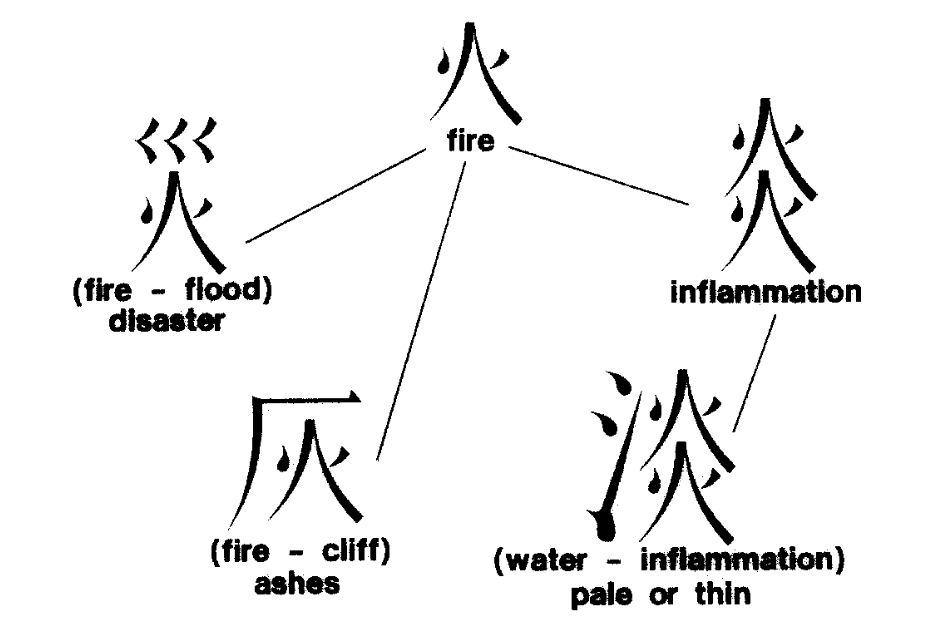
\includegraphics[width=0.7\linewidth]{figures/placeholders/icons_tree_structure}
	\caption{Hierarchically abstract icons (Redrawn from \parencite{blatter_earcons_1989})}
	\label{fig:iconstreestructure}
\end{figure}

There is no clearly superior choice. \parencite{gaver_sonicfinder:_1989} addresses representational earcons as \textit{auditory icons} and argues that this approach brings implicit benefits by exploiting the natural way we as humans react to sound. 
However, \parencite{blattner_earcons_1989} conclude that even though auditory icons are easily distinguishable and mappable, the main benefits of their application would be in systems with few distinct sounds: for $n$ different events $n$ mappings have to be memorized.
On the other hand, abstract earcons, while baring no intuitive relation to the event, require less mappings to be memorized due to their modularity: for $n$ different events, where $pq=n$, and $p$ and $q$ are distinct, unrelated elements, $p+q$ mappings have to be memorized.
% TODO: additionally, auditory icons need to be in their original ecology, and even then the mapping has to be learned. Even though that would be slightly more intuitive than learning abstract earcons.

\paragraph[Bridge]{}
Having reviewed the sound-related topics, which are relevant at the perception stage, it is time to take a look at the cognition stage of the information processing loop.
% TODO: situation awareness, actually, resides in both perception and cognition stages.


\begin{comment}
%(really small chapter, explaining the possible ways to implement auditory cues [auditory icons, earcons, …])

% Reference list
%% The Sonification Handbook

%% Sandell Kramer's book review
Sonification - The citation "non-speech audio to convey or perceptualize data"
%% Blattner. Earcons and icons

%% ? 3D User Interfaces

%% ? Kronland-Martinet, Real-time perceptial simulation of moving..

%% BBC Year Book
"The Symbolic, Evocative [bringing strong memories, images, or feeling to mind] Effect; e.g. the churning rhythm record used to express the confusion of a charwoman's mind in "Intimate Snapshots "; the use of sea sounds between all scenes in "The Flowers are not for You to Pick," expressing the inevitability of disaster."
%% Sound Immersion in First-Person Shooter


% TODO: also cite Gutwin 2002: the pre-research and the findings (the limitations of audio awareness, and "How and why does audio improve awareness?")
% TODO: maybe cite Gutwin 2011, too. THere was something on sound being a good tool or wharevs

Previous chapters implicitly established that auditory cues could potentially be a great way for providing awareness about the workspace. In this chapter I review sonification and the means it provides us with that can be utilized for interpretation of certain events or data. Sonification is a concept akin to visualization. Both can be applied to data, and while the visualization will do it in a visual form, sonification will use "non-speech audio to convey or perceptualize data".

\section{Sound Properties}
% I mention timbre in Experiments chapter
% + harmonics & halftones (and how they allow to differentiate between sounds), fundamental frequency
% Occlusion in audio SDKs
% 

% TODO: explain them here, but use as an example in later chapters. Potentially, like the chapter before
% HRTFs and stuff? Can tie the stereo headphones here as a exapmle of why they suck.

	
\section{Auditory Icons}
\section{Earcons}
\section{Summary}

Bridge: In the next chapter we will combine the knowledge from the previous chapters to …

\end{comment}